\chapter{Object Detection}
L'Object Detection è un \textit{task} legato al mondo della \textit{computer vision}
che consiste nel rilevare e classificare istanze di oggetti in immagini o video.

Negli ultimi anni, grazie soprattutto all'avvento delle \ac{gpu}, c'è stato un 
incremento notevole del potere computazionale. Questo ha portato a sviluppare tecniche 
sempre più raffinate allo scopo di raggiungere prestazioni sempre migliori. 

Sempre grazie allo sviluppo di hardware sempre più potente l'interesse sta sempre 
più virando verso il mondo del \textit{Deep Learning}. 
In questo capitolo cercheremo di classificare le varie metodologie con cui si 
porta a compimento la \textit{Object Detection}. 
La letteratura sui detector è molto disomogenea e variegata, prenderemo quindi come riferimento i lavori di 
\textit{Licheng Jiao, Fan Zhang, Fang Liu, Shuyuan Yang, Lingling Li, Zhixi Feng and Rong Qu} 
\cite{DBLP:journals/corr/abs-1907-09408} e 
\textit{Zhengxia Zou, Zhenwei Shi, Yuhong Guo and Jieping Ye} \cite{DBLP:journals/corr/abs-1905-05055}.


\section{Storia della object detection}
\label{sec:history_obj}
Una prima, ma importante distinzione va fatta tra il periodo pre e post \textit{deep learning}. Il primo periodo va dagli inizi degli anni $2000$ fino al $2014$. Il secondo periodo, dove hanno preso il sopravvento tecniche basate sul \textit{deep learning}, va dal $2014$ fino ai nostri giorni. Quest'ultime tecniche possono essere a loro volta divise in altre due categorie, \textit{One Stage Detector} e \textit{Two Stage Detector} (sarà il caso di tradurre in italiano?) il cui sviluppo procede in maniera parallela. In Figura \ref{fig:history_object_detection} è presente uno schema riassuntivo con tutte le pietre miliari raggiunte durante lo sviluppo di tecniche per il rilevamento di oggetti.
\begin{figure}
    \centering
    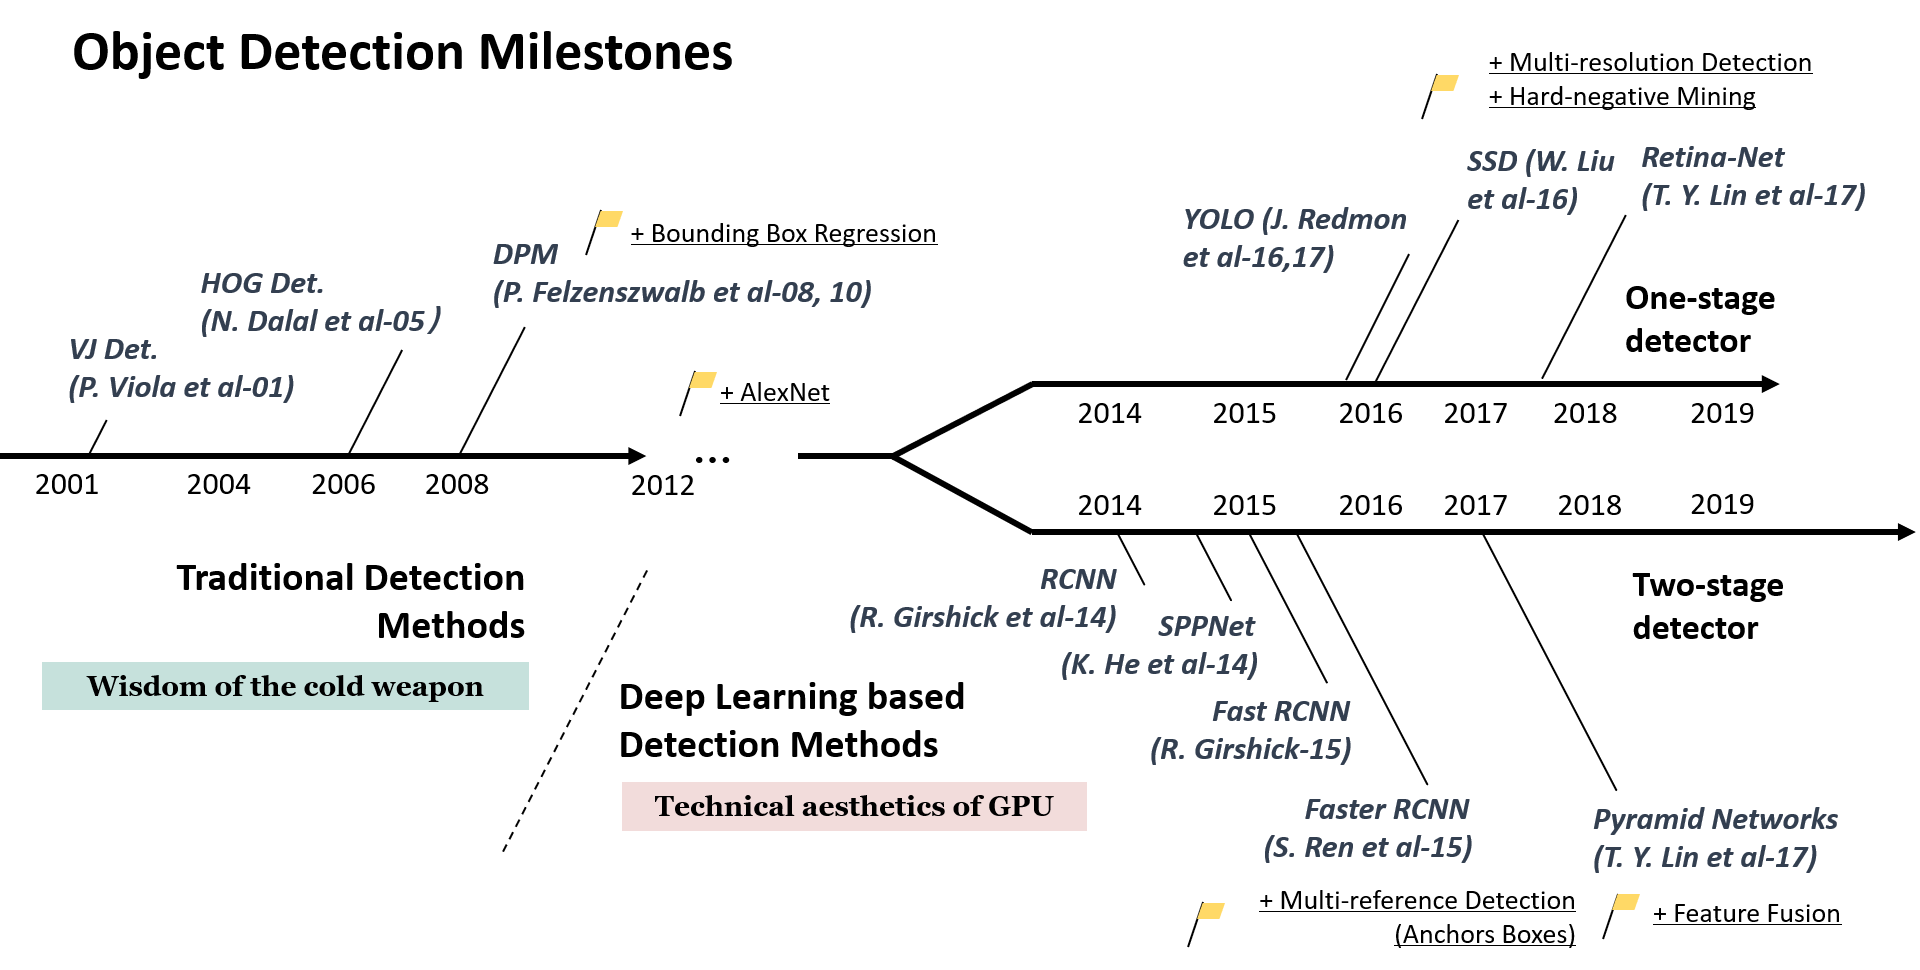
\includegraphics[width=\textwidth]{images/mile-stones.png}
    \caption{Storia della Object Detection \cite{DBLP:journals/corr/abs-1905-05055}}
    \label{fig:history_object_detection}
\end{figure}
\subsection{Evoluzione delle tecniche}
Durante questo ventennio i detector più famosi sono stati costruiti usando come mattoncini delle tecniche sviluppate ed affinate via via nel tempo. Queste tecniche sono di diverso tipo ed hanno subito evoluzioni di cui faremo una disamina nel proseguio di questa sottosezione.
\subsubsection{Prime tecniche}
Storicamente una delle prime tecniche si basava sul una teoria cognitiva chiamata \textit{Recognition by Components} \cite{biederman1987recognition}, ed è stata per molto tempo la base di alcuni lavori riguardanti il riconoscimento di immagini e la rilevazione di oggetti \cite{felzenszwalb2008discriminatively} \cite{fischler1973representation} \cite{leibe2008robust}.   

Nel passato alcuni ricercatori hanno formulato soluzioni al problema usando misure di similarità tra le componenti di un oggetto, tra la forma o i contorni, tra cui \textit{Distance Transforms} \cite{gavrila1999real}, \textit{Shape Contexts} \cite{belongie2002shape} e \textit{Edgelet} \cite{wu2005detection}.

I risultati iniziali erano molto promettenti, tuttavia quando la rilevazione è diventata più complicata queste tecniche hanno iniziato a mostrare i propri limiti, motivo per cui il passaggio al Machine Learning è stato quasi naturale. Le prime metodologie basate su questo approccio risalgono ad un periodo inquadrabile prima del $1998$, in questo caso la detection si basava su modelli statistici costruiti sopra le apparenze degli oggetti da rilevare. 
Il primo di questi modelli statistici nasce nel $1991$, chiamato \textit{Eigenfaces} \cite{turk1991eigenfaces} \cite{pentland1994view}, riesce in laboratorio a riconoscere volti in tempo reale.

Successivamente, fino al $2005$, l'evoluzione ha portato a tecniche in cui si cambiava radicalmente la rappresentazione, intesa come feature, delle immagini. Lo scopo era quindi apprendere come trasformare un immagine da insieme di pixel a insieme di coefficenti \textit{wavelet}. Grazie alla sua efficienza, tra tutte le trasformate, quella a prendere piede fu la \textit{Haar wavelet}. Dal $2005$ al $2012$ c'è stato un passaggio a rappresentazioni basate sul gradiente. 

Intorno al $1990$ iniziano a fare capolino le prime \ac{CNN} \cite{vaillant1994original} le quali però non hanno avuto grandi applicazioni per via dell'elevato costo computazionale rispetto alle risorse disponibili ai tempi. I modelli realizzati con \ac{CNN} non potevano essere quindi molto profondi, e per questo avevano forti limitazioni. Per ridurre questo elevato costo computazionale sono stati effettuati miglioramenti come \textit{space displacement network} \cite{lecun1998gradient}. Tramite questi perfezionamenti si è arrivato ad estendere ogni layer della \ac{CNN} in maniera tale da riuscire ad estrarre le feature da un immagine in un solo passaggio. Queste possono essere considerate un po' le antenate di quelle che attualmente chiamiamo \ac{FCN} \cite{long2015fully} \cite{chen2014semantic}. 
\subsubsection{Detection multiscala}
\label{subsec:multiscale_detection}
Uno degli aspetti più interessanti della ricerca si basa sulla rilevazione di oggetti con diverse misure o diverse proporzioni. Come è possibile bedere in Figura \ref{fig:multi_scale_history} la soluzione a questo problema ha attraversato varie fasi.
\begin{figure}
    \centering
    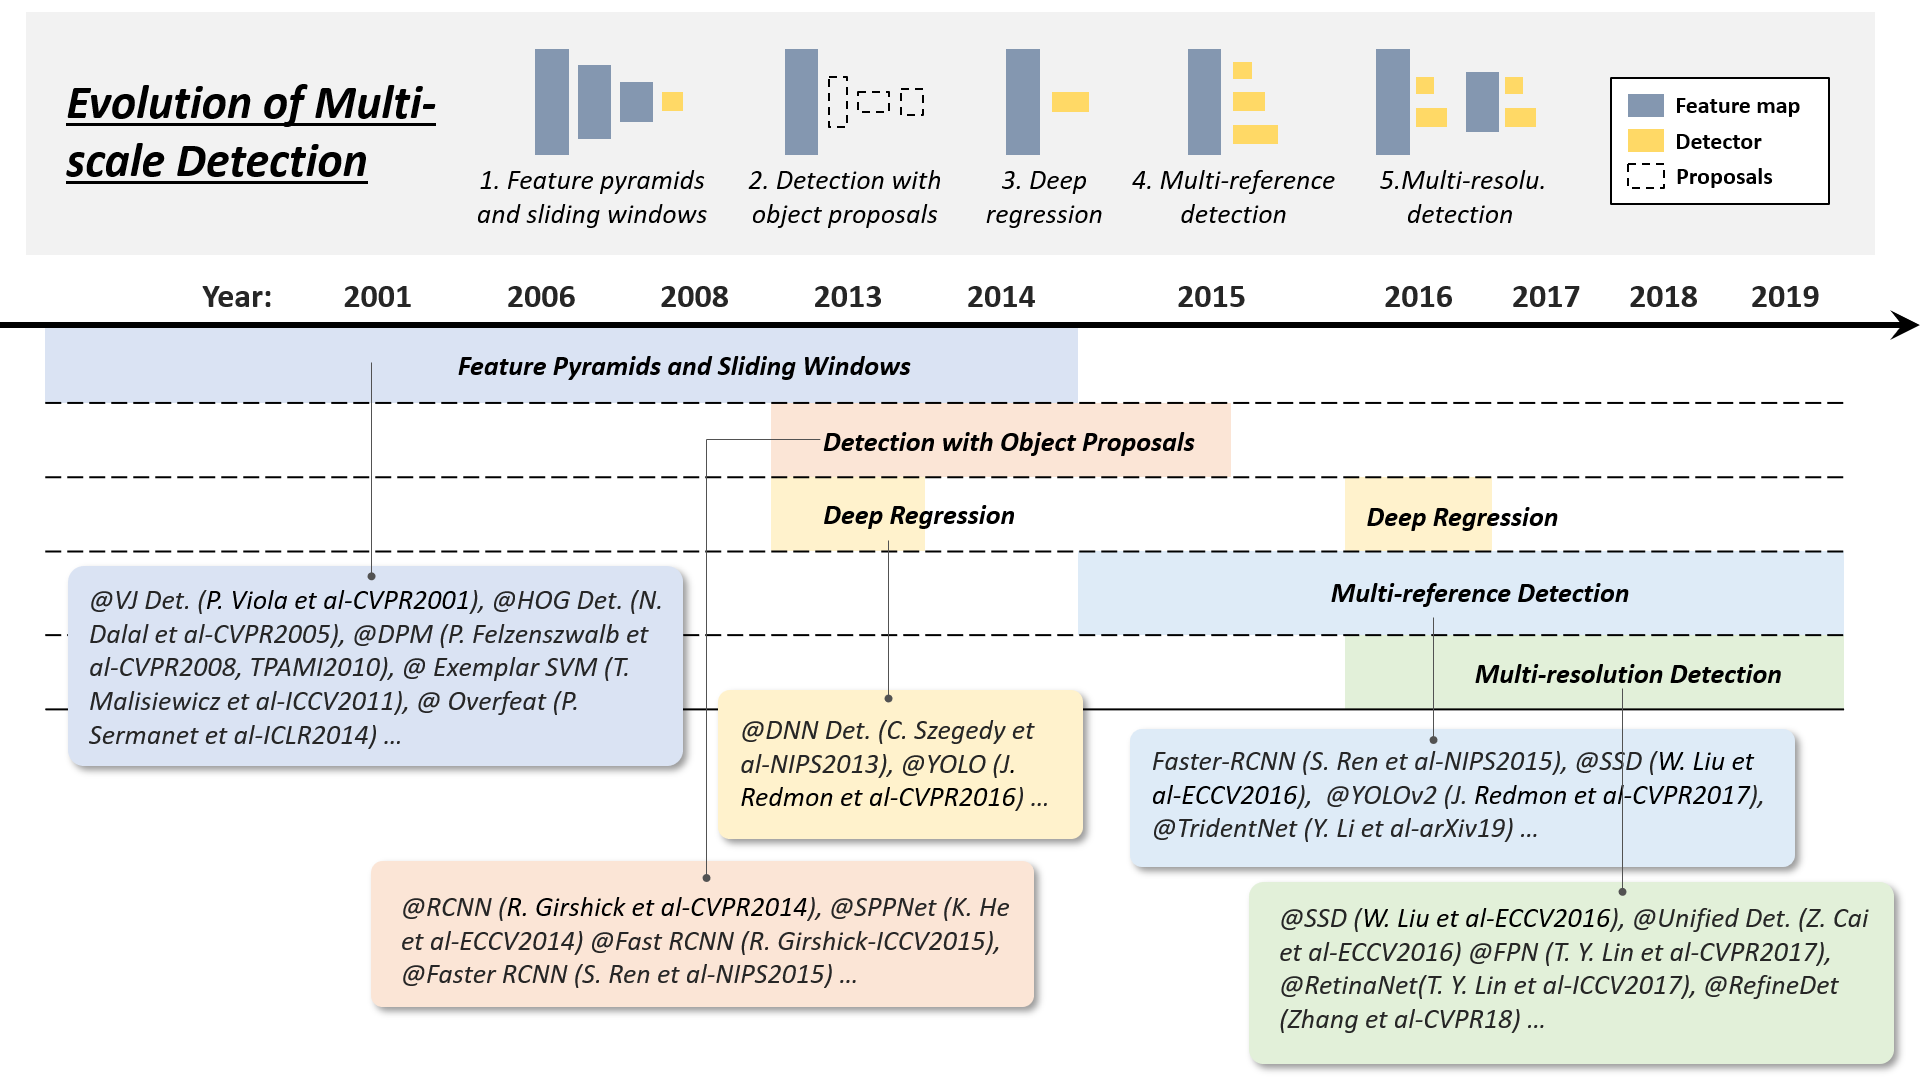
\includegraphics[width=\textwidth]{images/evol-multiscale.png}
    \caption{Evoluzione della detection multiscala \cite{DBLP:journals/corr/abs-1905-05055}}
    \label{fig:multi_scale_history}
\end{figure}
\paragraph{Feature piramidali e finestre scorrevoli}
L'idea dietro questa tecnica è abbastanza basilare, infatti dopo aver estratto le feature da un'immagine quello che viene fatto è far scorrere una finestra rettangolare di dimensione generalmente fissa per effettuare il rilevamento e la classificazione di oggetti. 

Dal $2004$ al $2014$ sono stati creati un sacco di detector basati su questa filosofia, il problema è che erano stati disegnati con l'intento specifico di rilevare oggetti con proporzioni fisse. Ricercatori come R. Girshick \textit{et al.} iniziarono a cercare soluzioni a questo problema, arrivando a formulare un modello mistura \cite{felzenszwalb2009object} composto da più modelli addestrati su oggetti con differenti proporzioni. Sono state sviluppate anche altre soluzioni, basate questa volta sull'addestrare modelli separati per ogni istanza di oggetto dell'insieme di addestramento \cite{malisiewicz2011ensemble} \cite{malisiewicz2011exemplar}. Le limitazioni di tutte queste tecniche risidono nel fatto che i dataset più moderni sono molto diversificati, quindi nel corso del tempo queste tecniche sono diventate sempre meno precise ed utilizzabili. Ciò ha portato allo sviluppo di \textit{Object Proposal}.
\paragraph{Object Proposal}
Il primo avvistamento di \textit{Object Proposal} risale al $2010$ in un task di rilevazione di oggetti \cite{alexe2010object}.
Possiamo definire una regione come un'area di un immagine contenente pixel che hanno caratteristiche comuni tra di loro. L'idea dietro questa tecnica è creare regioni non etichettate con classi che potenzialmente possono contenere qualunque tipo di oggetto, e lo scopo è riuscire a rilevare oggetti di varie misure e scale pur non dovendo necessariamente svolgere una ricerca esaustiva con finestre scorrevoli.

Per ottenere queste regioni di pixel su un immagine ci sono vari modi, discussi in parte da J. Hosang \textit{et al.} in \cite{hosang2015makes}.
\paragraph{Deep Regression}
Questa tecnica, sviluppata dal $2013$ al $2016$ si basa sull'idea di predirre direttamente le coordinate della \ac{BB} contenente l'oggetto usando come feature quelle estratte da un modello di \textit{deep learning} \cite{redmon2016you}. Il vantaggio fondamentale di questo approccio è l'efficienza e la velocità di implementazione, mentre uno svantaggio è la bassa accuratezza di localizzazione specialmente su piccoli oggetti.
\paragraph{Multi Reference Detection}
Questo approccio è il più usato per il rilevamento di oggetti con scale differenti e si basa sull'uso di un insieme di finestre rettangolari, che possono variare in dimensione e proporzioni, applicate sull'immagine, dette anche \textit{Anchor Boxes} \cite{ren2015faster, liu2016ssd, redmon2017yolo9000}. Sulla base di queste regioni rettangolari viene poi effettuata una predizione della \ac{BB}. 
\paragraph{Multi Resolution Detection}
Negli ultimi anni un altro approccio che ha preso piede si basa sul rilevare oggetti di con dimensioni differenti a layer differenti \cite{liu2016ssd, lin2017feature, zhang2018single, cai2016unified}. Basti pensare alle \ac{CNN} che nel corso della propagazione dell'immagine in input, grazie alla loro composizione, formano una serie di feature piramidali. Diventa quindi più facile rilevare oggetti grandi nei layer più profondi e viceversa diventa più facile rilevare oggetti piccoli nei layer meno profondi. 
\subsubsection{Regressione basata su Bounding Box}
Questo insieme di metodologie ha lo scopo di affinare la posizione delle \ac{BB} basandosi sulle rilevazioni effettuate tramite \textit{Object Proposal} o \textit{Anchor Boxes}, descritte in \ref{subsec:multiscale_detection}. Uno schema riassuntivo dell'evoluzione tecnica di questi approcci è in Figura \ref{fig:bbox_history}.
\begin{figure}
    \centering
    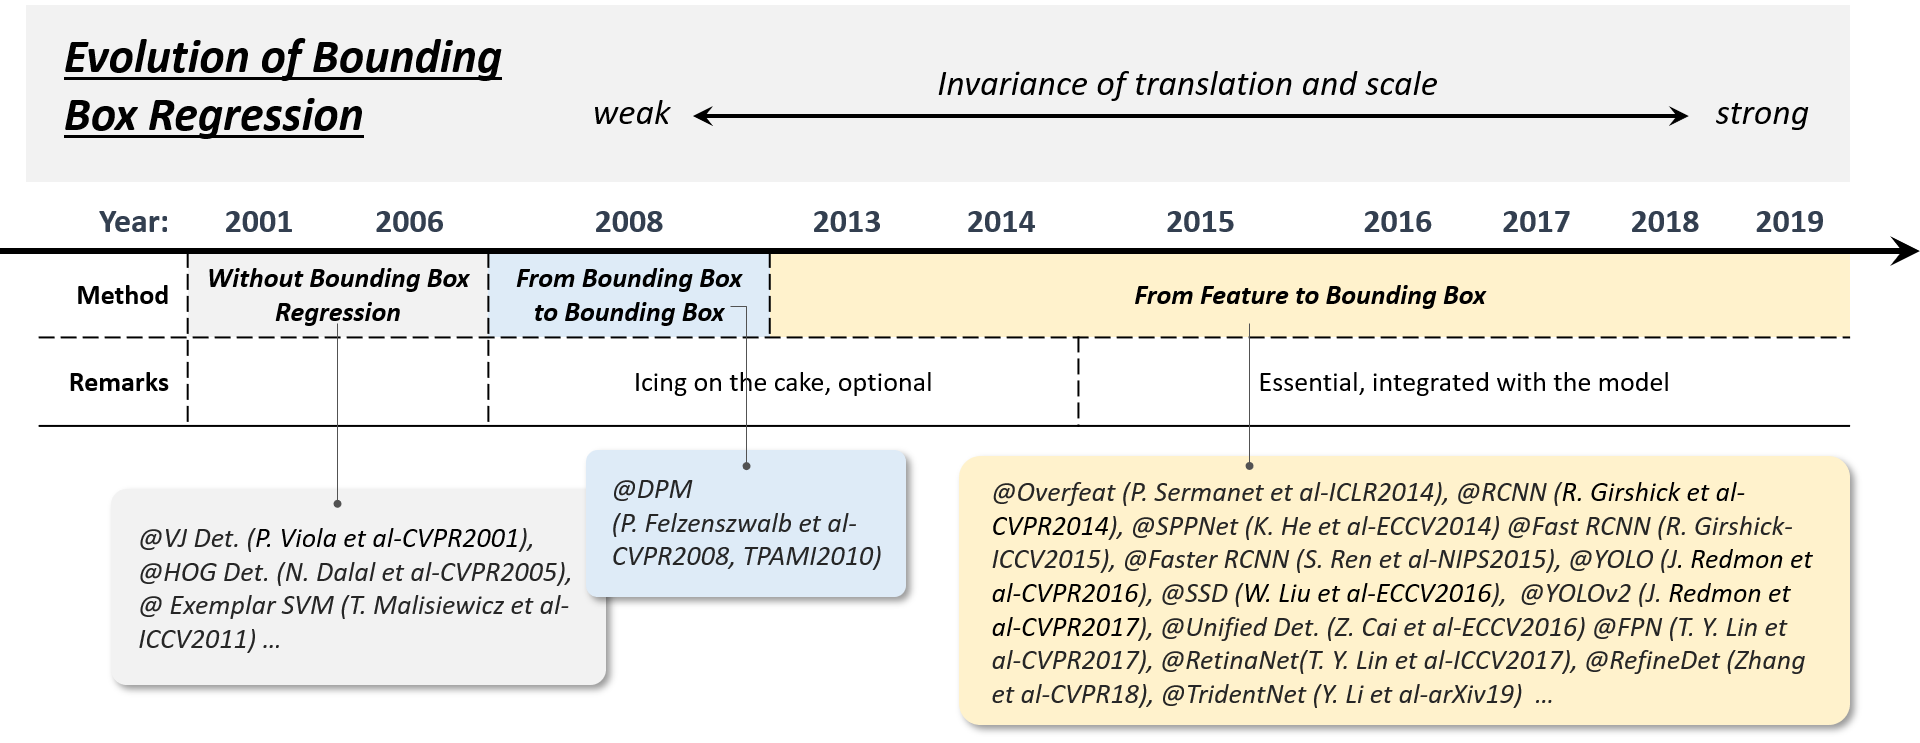
\includegraphics[width=\textwidth]{images/evol-bbreg.png}
    \caption{Evoluzione della regressione basata su \ac{BB} \cite{DBLP:journals/corr/abs-1905-05055}}
    \label{fig:bbox_history}
\end{figure}
I primi detector non raffinavano in alcun modo la posizione delle \ac{BB}, anzi molte volte usavano direttamente l'output derivato da un algoritmo basato su finestre scorrevoli. L'unico modo per ottenere rilevazioni più precise era quindi costruire modelli piramidali molto densi e assicurarsi di far scorrere la finestra lungo tutta l'immagine.
\paragraph{Da Bounding Box a Bounding Box}
I primi ad usare una forma di regressione per aumentare la precisione sulle \ac{BB} sono stati P. F. Felzenszwalb \textit{et al.} in DPM \cite{5255236} formulando la soluzione con il metodo dei minimi quadrati. Per scendere più nel dettaglio dobbiamo considerare un modello con feature piramidali.
Nel modello proposto in \cite{5255236} viene usata l'intera configurazione di $z$ per predirre la \ac{BB} riguardante quell'oggetto. In breve l'implementazione è effettuata tramite una funzione $g(z)$ che restituisce come output le coordinate $(x_1, y_1)$ e $(x_2, y_2)$ della \ac{BB}. Dopo la fase di addestramento del modello viene usato l'output di $g(z)$ per un'ulteriore fase di addestramento dove tramite il metodo dei minimi quadrati si impara a predirre $x_1, y_1, x_2 \text{ e } y_2$ partendo da $g(z)$. C'è da specificare che questo tipo di ottimizzazione è stato implementato a livello di post-processing, quindi risulta del tutto opzionale.
\paragraph{Da feature a Bounding Box}
A differenza del tipo di ottimizzazione proposto in precedenza, con l'introduzione delle \textit{Faster RCNN} \cite{ren2015faster} nel $2015$ la regressione è implementata a livello di rilevamento dell'oggetto e quindi viene addestrata insieme al modello. Inoltre, sempre confrontandolo con quanto detto prima, vengono usate anche diverse funzioni di loss da minimizzare che risultano più robuste rispetto a quella usata nei minimi quadrati. Degli esempi possono essere la \textit{smooth-L1} o la \textit{root-square}.

\subsubsection{Valutazione del contesto}
Generalmente gli oggetti che vengono rilevati dai sistemi di detection sono immersi in un contesto. Il cervello umano durante la fase cognitiva trae vantaggio dal riconoscere un contesto, motivo per cui le tecniche spiegate nel proseguio di questa sottosezione provano a emulare questa capacità degli umani. Una breve storia di come queste tecniche si sono evolute è in Figura \ref{fig:context_history}.
\begin{figure}
    \centering
    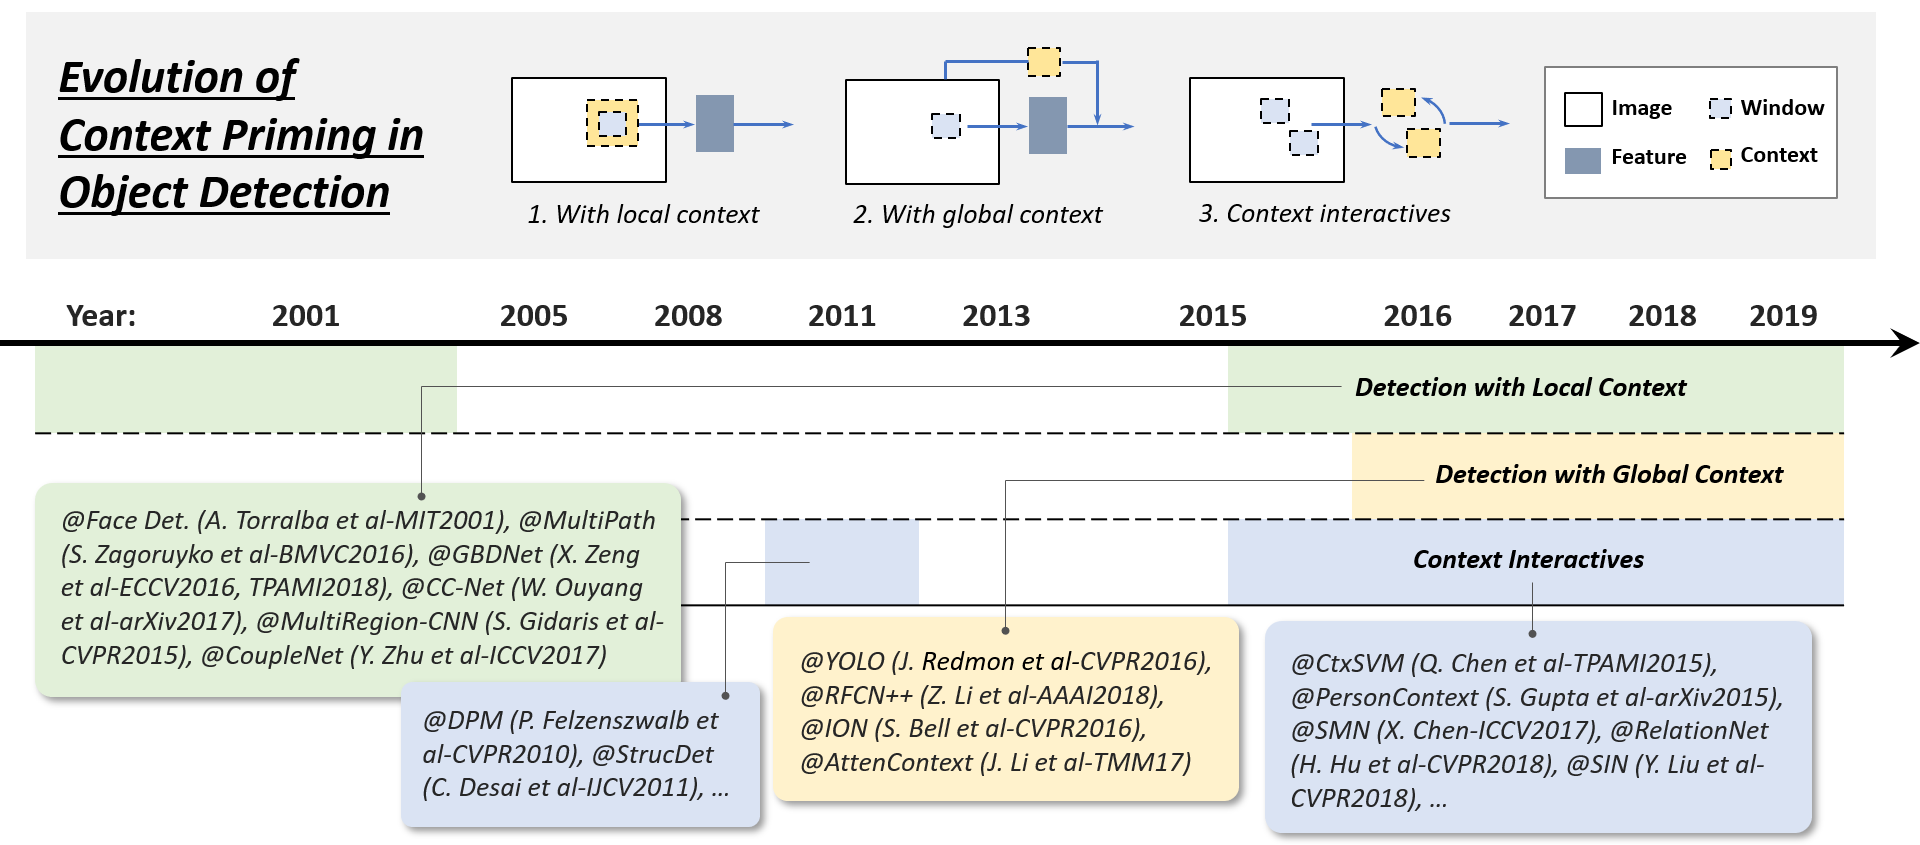
\includegraphics[width=\textwidth]{images/evol-context.png}
    \caption{Evoluzione del context priming \cite{DBLP:journals/corr/abs-1905-05055}}
    \label{fig:context_history}
\end{figure}
\paragraph{Contesto locale}
Per contesto locale si intendono tutte le informazioni visive che fanno parte dell'area prossima ai contorni di un oggetto. Sin dagli anni 2000 Sinha e Torralba in \cite{torralba2001detecting} hanno provato che includere del contesto locale migliora le prestazioni ai fini del rilevamento di volti. Dalal e Triggs in \cite{dalal2005histograms} hanno dimostrato che introdurre una piccola porzione di sfondo migliora i risultati anche nel rilevamento dei pedoni. 
\paragraph{Contesto globale}
Il contesto globale può essere considerato come una fonte di informazione aggiuntiva riguardante la scena in cui l'oggetto da rilevare è immerso. Un metodo usato all'inizio per inglobare nella detection informazioni sul contesto globale era realizzare delle statistiche che riassumevano la totalità degli elementi compresi nella scena \cite{divvala2009empirical}. In lavori più moderni catalogabili come modelli di \textit{deep learning} sono state intraprese due strade, la prima è quella di inglobare il contesto tramite campi recettivi sempre più ampi, a volte anche più dell'immagine stessa \cite{redmon2016you} o  usare l'operazione di \textit{pooling} delle \ac{CNN} \cite{li2018r}. La seconda via per ottenere informazioni dal contesto globale è pensare ad esso come un flusso di informazioni sequenziali ed usare \ac{RNN} \cite{bell2016inside, li2016attentive}. 
\paragraph{Contesto derivato dalle interazioni}
L'ultima contestualizzazione che si può dare ad un oggetto riguarda le sue interazioni con ciò che lo circonda. Per interazioni si possono intendere tutte quei vincoli o dipendenze che può avere l'obbiettivo della rilevazione. Recentemente in alcuni lavori sono state analizzate questo tipo di informazioni contestuali ai fini del miglioramento della detection. Questi miglioramenti possono essere divisi in due macrocategorie, la prima di queste è quella in cui si esplorano le relazioni tra oggetti individuali \cite{felzenszwalb2009object, desai2011discriminative, song2011contextualizing, chen2017spatial, hu2018relation}. Nella seconda categoria fanno parte i lavori nei quali vengono prese in considerazione le relazioni che ci sono tra gli oggetti e la scena che li circonda \cite{gupta2015exploring, liu2018structure}.
\subsubsection{Non Maximum Suppression}
Per \ac{NMS} si fa riferimento a tutte quelle tecniche di post processing per ridurre il fenomeno delle \ac{BB} duplicate. Questo fenomeno si concretizza quando, per la stessa rilevazione, ci sono più \ac{BB} che lo circondano con confidenze molto simili tra di loro. L'evoluzione di queste tecniche nel corso del tempo è possibile vederla in Figura \ref{fig:NMS_history}. 
\begin{figure}
    \centering
    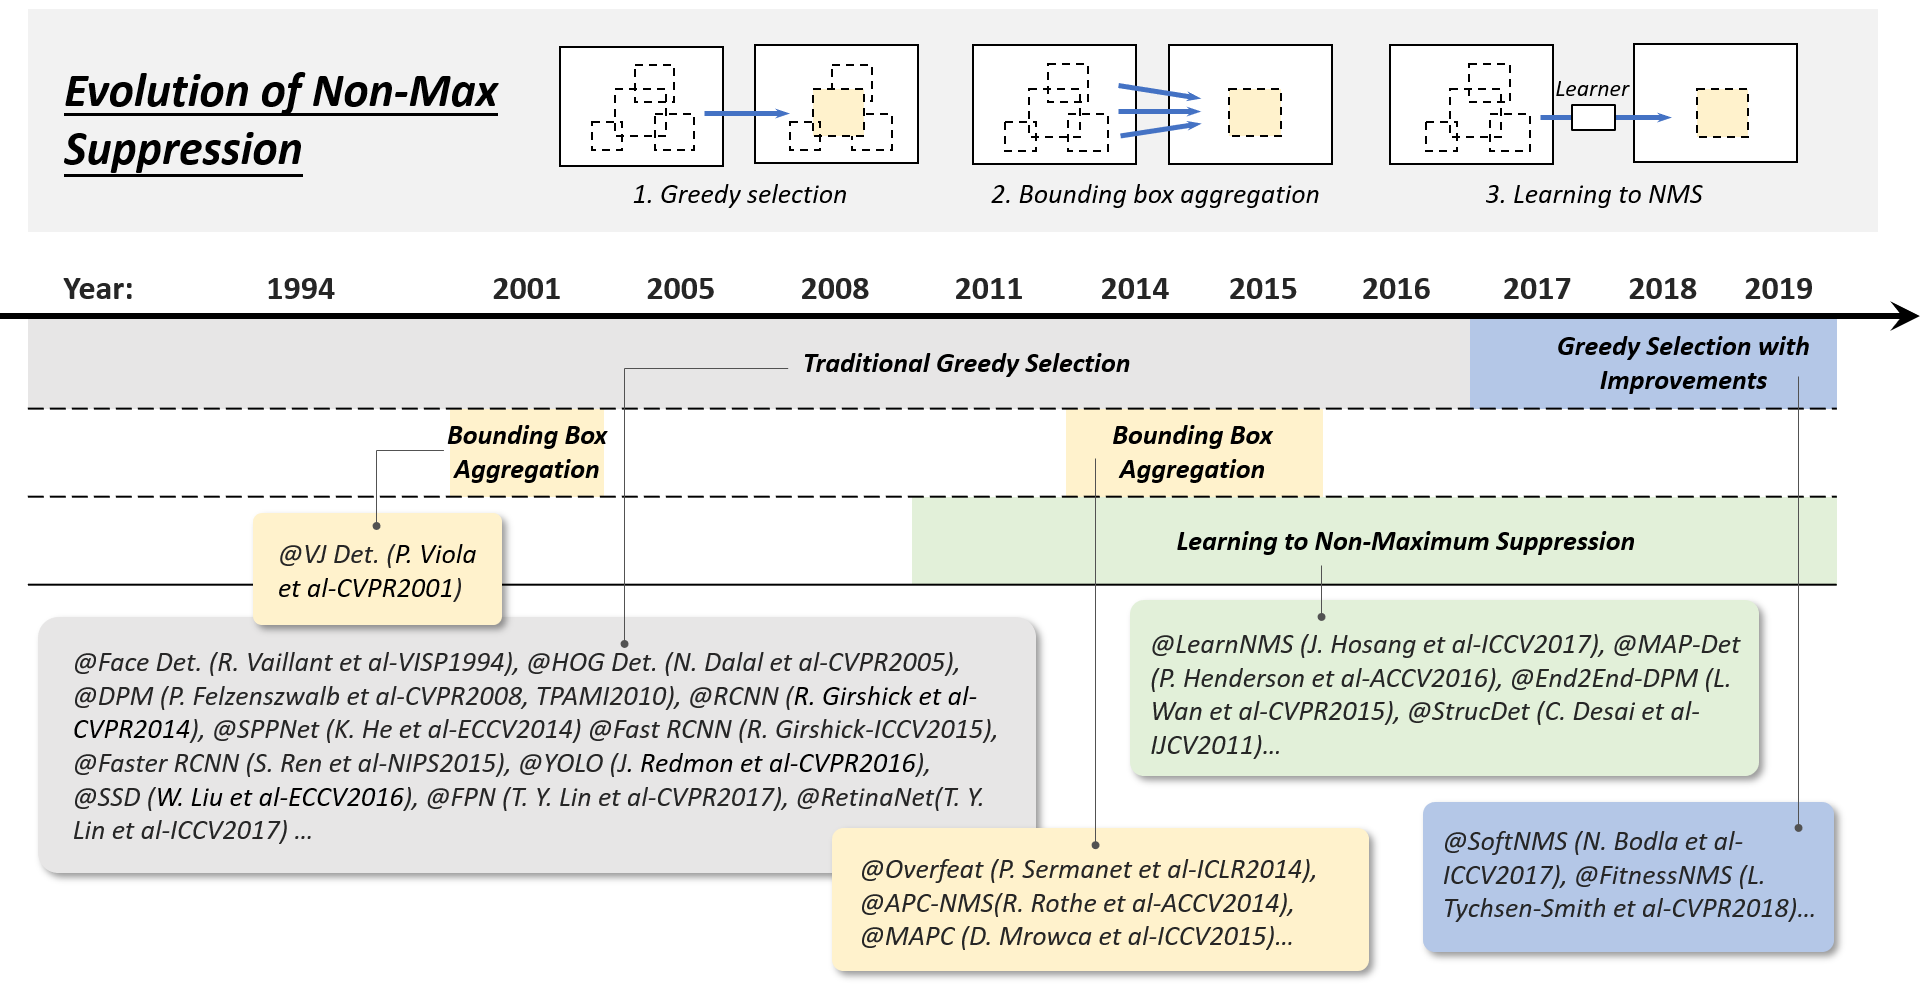
\includegraphics[width=\textwidth]{images/evol-nms.png}
    \caption{Evoluzione della Non Maximum Suppression \cite{DBLP:journals/corr/abs-1905-05055}}
    \label{fig:NMS_history}
\end{figure}


\paragraph{Greedy}
La maniera più semplice per attuare la \ac{NMS} è con un algoritmo di tipo \textit{greedy}, infatti per un insieme di \ac{BB} sovrapposte si considera solamente quella con la confidenza massima, mentre le altre vengono scartate. La sua semplicità, che da un certo punto di vista può anche essere vista come un punto di forza, può anche essere fonte di debolezze in quanto un algoritmo \textit{greedy} non sempre porta all'ottimalità. Si possono infatti verificare casi in cui la \ac{BB} con massima confidenza non ricopre tutto l'oggetto, o ancora peggio le \ac{BB} di oggetti vicini tra di loro possono essere scaratate erroneamente.


\paragraph{Aggregazione di Bounding Box}
L'aggregazione di \ac{BB} vicine tra di loro è un altro approccio per attuare la \ac{NMS} \cite{viola2001rapid, sermanet2013overfeat, rothe2014non, mrowca2015spatial}. L'aggregazione può essere fatta sia attraverso algoritmi di \textit{clustering}, sia combinando le \ac{BB} sovrapposte in un unica singola detection. 


\paragraph{Imparare ad applicare Non-maximum Suppression}
Approcci più recenti per migliorare le già sopracitate tecniche di \ac{NMS} riguardano l'apprendimento automatico \cite{wan2015end, desai2011discriminative, hosang2017learning, henderson2016end}. L'idea dietro questi metodi è trattare la \ac{NMS} alla stessa stregua di un filtro che assegna nuovi valori di confidenza a tutte le detection e quindi bisognoso di una fase di addestramento. 

\subsubsection{Hard Negative Mining}
Uno dei problemi a cui bisogna far fronte quando si tratta la \textit{Object Detection} è lo sbilanciamento tra gli oggetti che vogliamo rilevare e conseguentemente classificare e tutto quello che non ci interessa. La prima soluzione che potrebbe venire in mente per risolvere questo problema è addestrare il modello a riconoscere lo sfondo, ma questo porta a risultati distruttivi durante l'addestramento in termini di efficienza. Tecniche di \ac{HNM} servono proprio a risolvere queste problematiche. Una breve storia è possibile vederla in Figura \ref{fig:HNM_history}.
\begin{figure}
    \centering
    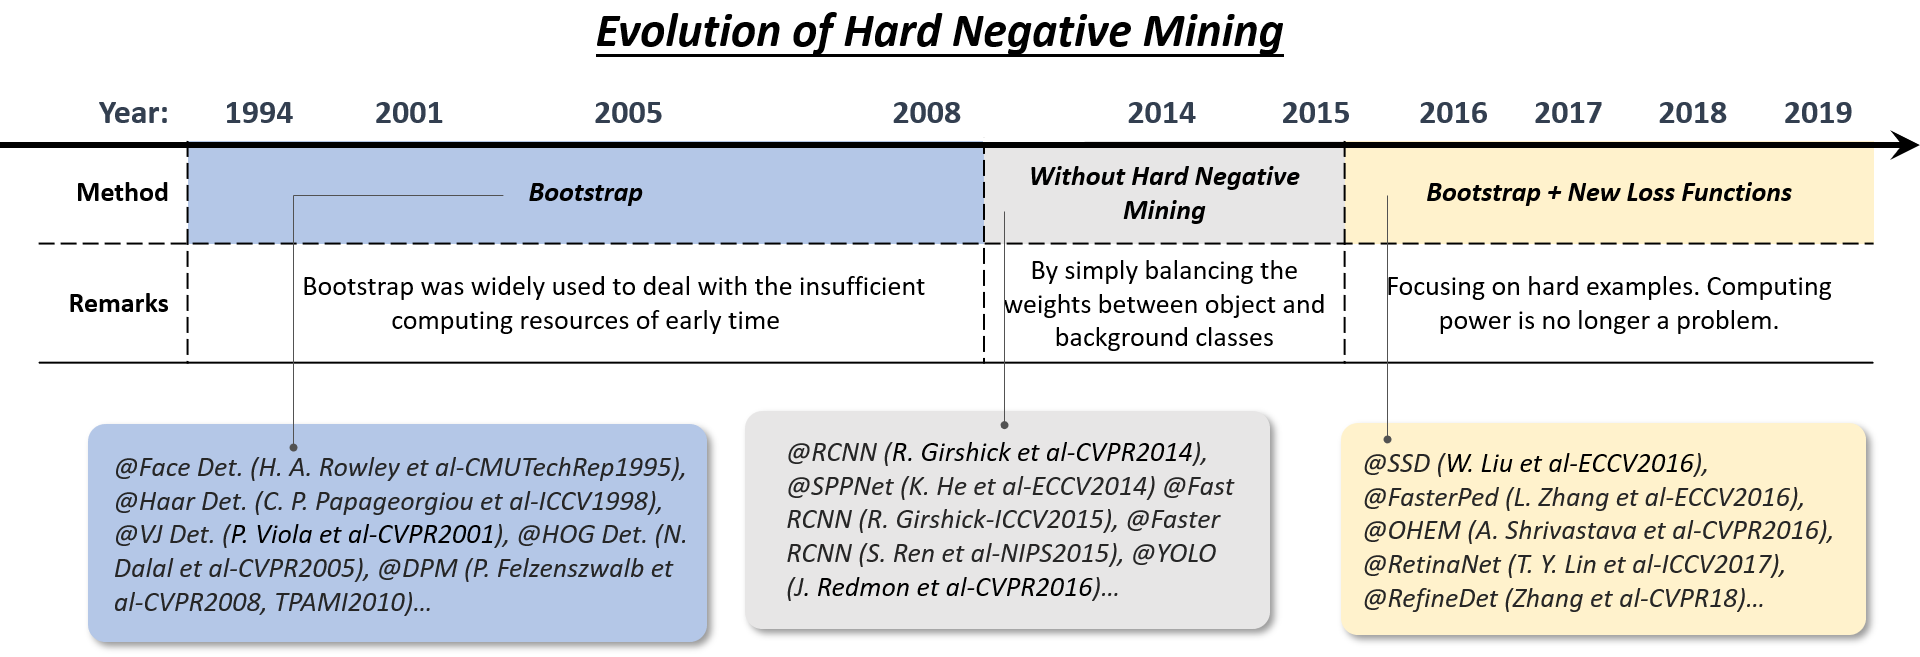
\includegraphics[width=\textwidth]{images/evol-hardnegmining.png}
    \caption{Evoluzione di Hard Negative Mining \cite{DBLP:journals/corr/abs-1905-05055}}
    \label{fig:HNM_history}
\end{figure}
\paragraph{Bootstrap}
Per Bootstrap si fa riferimento ad un gruppo di tecniche attraverso le quali si fa iniziare la fase di addestramento prendendo con dello sfondo. Successivamente quando si rilevano esempi di sfondo classificati erroneamente si aggiungono al processo di addestramento. Questo approccio risulta efficiente in quanto si evita di addestrare il modello su milioni di esempi di sfondi \cite{viola2001rapid, papageorgiou1998general, rowley1996human}.
\paragraph{HNM in detector basati su deep learning}
Recenemente modelli come Faster RCNN e \ac{YOLO} per risolvere questo problema bilanciano i pesi tra finestre con esempi negativi e positivi. Nonostante tutto però non viene risolto completamente il problema di sbilanciamento, quindi c'è stato un ritorno al \textit{bootstrap}. Un altro modo per risolvere lo sbilanciamento è l'introduzione di nuove funzioni di Loss, come ad esempio la Focal Loss in RetinaNet \cite{lin2017focal}. 
\subsection{Dataset}
L'insieme dei dati con cui addestrare e testare le performance dei modelli via via sviluppati nel corso del tempo ha subito un evoluzione. Costruire dataset sempre più grandi e con meno bias è sempre stato un obbiettivo principale che si ponevano i ricercatori, tutto ciò per realizzare dei benchmark che mettessero sempre di più a dura prova i nuovi modelli. Nel seguito di questa sezione analizzeremo in breve alcuni dei dataset più famosi nell'ambito della computer vision, con particolare attenzione per alcuni incentrati sulla rilevazione di pedoni. 
\paragraph{MIT Ped.} Risale all'inizio del nuovo milleno ed è uno dei primi dataset che ha come scopo il riconoscimento di pedoni. Rispetto agli standard odierni risulta molto piccolo in quanto contiene circa 509 immagini usabili per l'addestramento e 200 usabili per la fase di test. \cite{papageorgiou2000trainable} 
\paragraph{INRIA} Risalente al 2005, nasce dall'esigenza di creare un dataset dove la detection diventasse più complicata rispetto a quello fatto dal MIT \cite{dalal2005histograms}. Contiene 1805 immagini ad una risoluzione di $64 \times 128$ pixel di esseri umani. Le immagini usate per l'insieme di training sono 2478, ovvero 1239 immagini, contenenti esempi positivi, prese dal totale più le stesse immagini ma riflesse secondo l'asse delle $y$.

\paragraph{Pascal VOC}
\ac{VOC} è collocabile in un periodo che va dal $2005$ al $2012$ \cite{everingham2010pascal, everingham2015pascal}. \ac{VOC} consiste di due parti complementari, la prima è un dataset pubblico e disponibile per esperimenti e benchmark, la seconda è una sfida annuale. Nel corso degli anni ne sono state sviluppate diverse versioni, individuabili dal pattern VOC\texttt{ANNO}. I task effettuabili su questo dataset spaziano classificazione di immagini alla object detection passando anche per il rilevamento di azioni. 
Per la sfida nel $2007$ sono state raccolte solo immagini dal social network \href{https://www.flickr.com/}{Flickr}. Le immagini sono molto variegate, ad esempio come scritto nell'articolo di presentazione del dataset \cite{everingham2010pascal} ci possono essere motociclette in diverse pose e forme, come può essere il veicolo per strada o come soggetto principale del fotogramma. 
Un altro esempio è la classe \textit{"person"}, mentre in molti dataset con questa classe ci si riferisce ad un pedone in VOC2007 con questa classe si fa riferimento ad un essere umano in diversi contesti. 
Per realizzare il dataset sono state definite delle keyword con cui effettuare query su \href{https://www.flickr.com/}{Flickr}. Queste suddette keyword sono state definite sulla base delle classi degli oggetti che si desiderava annotare. Tramite queste query sono state recuperate $500.000$ immagini, non prendendo in considerazione la data di acquisizione, il nome del fotografo, la location e via discorrendo. 
Le query venivano effettuate a gruppi di $100.000$ immagini alla volta, di cui venivano selezionate casualmente solamente alcuni fotogrammi ed inseriti nel dataset. Questa operazione è stata ripetuta fino ad ottenere la quantità desiderata di file. 
L'operazione successiva è stata quella di eliminare i duplicati o comunque immagini molto somiglianti tra di loro, una volta fatto questo sono passati ad annotarle. Di queste $500.000$ immagini agli annotatori ne sono state presentate $44.269$. Gli annotatori avevano la facoltà di scartare alcune immagini se le ritenevano non adatte ad essere annotate o avevano una confidenza bassa sull'eventuale annotazione da effettuare. Nonostante ciò è stato scoperto un'elemento che portava a del bias all'interno del dataset. L'elemento in questione riguardava il modo in cui le immagini sono state recuperate. Quando si effettua una query su \href{https://www.flickr.com/}{Flickr} il server restituisce le immagini in ordine cronologico di upload sulla piattaforma. Il dataset è stato realizzato nel Gennaio $2007$, quindi buona parte delle immagini erano ambientate in un contesto natalizio o perlopiù invernale. Con VOC2008 il problema è stato risolto aggiungendo una data casuale all'interno della query per recuperare le immagini.  

\paragraph{Caltech Pedestrian Dataset} Il \textit{Caltech Pedestrian Dataset} \cite{dollar2009pedestrian} nasce nel 2009 ed è molto più ampio di tutti gli altri dataset visti in precedenza. Le immagini sono state ricavate da circa 10 ore di video girato a 30 frame al secondo in un ambiente urbano con traffico regolare. È quindi presente un numero di frame che è nell'ordine di grandezza di $10^6$. La telecamera con cui sono state acquisite le registrazioni è stata piazzata su un'autovettura con un guidatore che attraversava le strade di Los Angeles guidando in maniera normale. La risoluzione delle immagini è di $640 \times 480$ e come conseguenza del fatto che il sistema è stato più volte smontato e rimontato ci sono piccole variazioni nella posizione della telecamera. 

Sono stati annotati $250.000$ fotogrammi, per un totale di $350.000$ \ac{BB} e $2300$ pedoni univoci. Di tutti i fotogrammi, circa il $50\%$ non hanno pedoni, mentre il $30\%$ del totale ne ha almeno due. In media un pedone è visibile per un tempo di 5 secondi. Come su dataset più recenti i pedoni sono raggruppati secondo la loro distanza dal guidatore. In particolare abbiamo che i pedoni sono vicini se la loro altezza è maggiore di $80$ pixels, sono ad una distanza media se la loro altezza è compresa tra $30$ ed $80$ pixels, mentre sono consideati lontani se la loro altezza è al più $30$ pixels. Questa discretizzazione riguardante la distanza dei pedoni è stata realizzata seguendo la distribuzione delle altezze degli stessi all'interno del dataset. Sono state inoltre prese in considerazione statistiche riguardanti l'occlusione dei pedoni e la loro posizione rispetto alla telecamera.

Il dataset è stato creato da $11$ sessioni dove in ognuna di queste venivano esplorati $5$ quartieri. Dopodiché le prime sei sessioni sono state destinate all'addestramento, mentre le rimanenti cinque sono state adibite a test set.

\paragraph{KITTI}  \cite{geiger2012we} Questo dataset è realizzato a partire da hardware usato per la guida autonoma. La particolarità è che offre informazioni tridimensionali dell'ambiente grazie a dei sensori laser dedicati che mappano il territorio circostante. Per la realizzazione sono state quindi utilizzate due telecamere a colori con una risoluzione di $1392 \times 512$ pixels, uno scanner laser ed un localizzatore GPS con un'unità di correzione RTK, il tutto orchestrato da un calcolatore su cui girava un database in real time.  Tutto questo hardware è stato montato su una station wagon che è stata guidata per dei normali scenari cittadini. 
Inoltre le annotazioni non sono \ac{BB} in due dimensioni, ma bensì dei parallelepipedi che avvolgono gli oggetti. Per la loro realizzazione sono stati presi annotatori umani che hanno posizionato \ac{BB} tridimensionali su oggetti come auto, furgoni, camion, tram, pedoni e ciclisti. Inoltre gli annotatori sono stati istruiti per marcare ogni \ac{BB} come visibile, semi occlusa, occlusa o troncata. 



\paragraph{ILSVRC}
Come per \ac{VOC} anche \ac{ILSVRC} \cite{russakovsky2015imagenet} è una challenge organizzata annualmente dal $2010$ al $2017$. Inoltre, sempre come per \ac{VOC} è presente un dataset pubblico disponibile per addestramenti e test. 
Come per alcuni dei dataset precedentemente introdotti le immagini state prese in parte da Flickr, con l'aggiunta però di altri motori di ricerca. In particolare andremo ad analizzare la costruzione della parte di dataset riguardante la \textit{object detection}, però il dataset contiene anche una parte dedicata alla classificazione di immagini ed un'altra parte dedicata alla rilevazione singola di oggetti all'interno dell'immagine. 

Le classi di oggetti presenti sono $200$ e sono stati scelte partendo dalle $1000$ classi usate per la classificazione di immagini. Una prima riduzione per arrivare a $494$ classi è stata inizialmente effettuata tramite l'eliminazione di label corrispondenti ad oggetti che occupavano gran parte del fotogramma o semplicemente non adatti alla \textit{object detection}. Un ulteriore operazione di unificazione tra classi simili ha portato il numero a $200$. 

Per il training set le immagini hanno tre provenienze differenti. Le prima sorgente di immagini è la parte di dataset dedicata alla rilevazione singola di oggetti. Per aggiungere ulteriori esempi negativi sono state effettuate prese immagini da motori di ricerca. Le immagini provenienti da queste due prime fonti sono state annotate solamente con un sottoninsieme delle classi totali. L'ultima sorgente di immagini è la piattaforma Flickr su cui sono state fatte query generiche. 
Riguardo invece la porzione di dataset dedicata alla validazione e al test la situazione è molto simile in quanto la fonte primaria ($77\%$) è la porzione di di \ac{ILSVRC}2012 adibita alla rilevazione di oggetti singoli, a cui però sono state sottratte le immagini nel quale gli oggetti occupavano più del $50\%$ dell'area totale del fotogramma. Per aggiungere ulteriori esempi, come per il training set, sono state effettuate interrogazioni generiche su Flickr. A differenza dell'insieme di immagini di addestramento, per la validazione e il test, sono state usate tutte e $200$ le classi disponibili. 
In totale per il traning set sono presenti circa $458.000$ immagini, mentre per il validation e test set sono presenti $46.000$ fotogrammi. 
\paragraph{CityPersons} Zhang \textit{et al. } \cite{zhang2017citypersons} propongono un nuovo dataset derivante da Cityscapes \cite{cordts2016cityscapes}, ma invece che focalizzarsi sulla segmentazione delle scene in contesti urbani CityPersons è incentrato sulla rilevazione di pedoni. Infatti per ogni frame di Cityscapes sono stati annotati esseri umani tramite \ac{BB}.

Le classi usate in questo dataset sono quattro, e variano a seconda della postura del pedone. Con \texttt{pedestrian} vengono indicate le persone in piedi, che corrono o camminano, mentre con \texttt{rider} si indicano quelle persone che sono alla guida di un mezzo a due ruote. Sono presenti altre due classi per indicare le persone sedute (\texttt{sitting person}) e persone con pose inusuali (\texttt{other person}).

Viene standardizzato il processo di annotazione dei \texttt{pedestrian} e \texttt{riders} in quanto le \ac{BB} hanno tutte la stessa proporzione ($0.41$), è quindi sufficiente tracciare una linea che va dalla testa ai piedi del pedone per generare una \ac{BB} delle giuste dimensioni. In questo modo si perfeziona l'allineamento della regione con l'oggetto da rilevare, e quindi si migliorano le prestazioni dell'eventuale modello. 
Per le rimanenti due classi invece non è stato standardizzato il processo, quindi vengono semplicemente disegnate \ac{BB} che contengono la persona. Un'altra operazione che è stata effettuata è stata ricercare tra le immagini tutte quelle \texttt{persone false} (manichini, statue, riflessi) per marcarli come regioni da ignorare. 

Il dataset è composto da $5000$ immagini, con un totale di circa $35000$ annotazioni e $13000$ regioni da ignorare. A differenza di KITTI e Caltech c'è una densità di persone per frame sette volte superiore ed il numero di individui distinti è prossimo a $20.000$, quindi rispettivamente $15$ e $3$ volte superiore.  La suddivisione tra test e train set è la stessa di Cityscapes. 
\paragraph{MS-COCO} \cite{lin2014microsoft}
Attualmente \ac{MSCOCO} grazie alla difficoltà di ottenere buone prestazioni è considerato uno dei più interessanti dataset per la \textit{object detection}. Rispetto a \ac{ILSVRC} ha meno classi, ma contiene molte più immagini ed annotazioni. Il punto di forza di questo dataset è la grande molteplicità di contesti in cui sono stati catturate le immagini e soprattutto la densità di oggetti che rispecchia in maniera del tutto similare quella del mondo reale. Inoltre una proprietà importante è che gli oggetti si trovano quasi sempre in contesti appropriati.

Andando più nello specifico ci si trova davanti ad un dataset che nella sua ultima versione ha, per la \textit{object detection}, circa $165.000$ immagini dedicate all'addestramento, e circa $160.000$ dedicate alla validazione ed al test. Le classi in totale sono $91$. In media ci sono $3.5$ categorie diverse e $7.7$ oggetti per immagine. In Figura \ref{fig:dataanalysis_coco} è presente uno schema riassuntivo delle statistiche di questo dataset, ed un altra cosa che si può notare è che, rispetto ad esempio a \ac{ILSVRC} e \ac{VOC}, ci sono molte meno immagini con una sola \ac{BB}, infatti in \ac{MSCOCO} solamente il $10\%$ rientra in questa categoria.
\begin{figure}
    \centering
    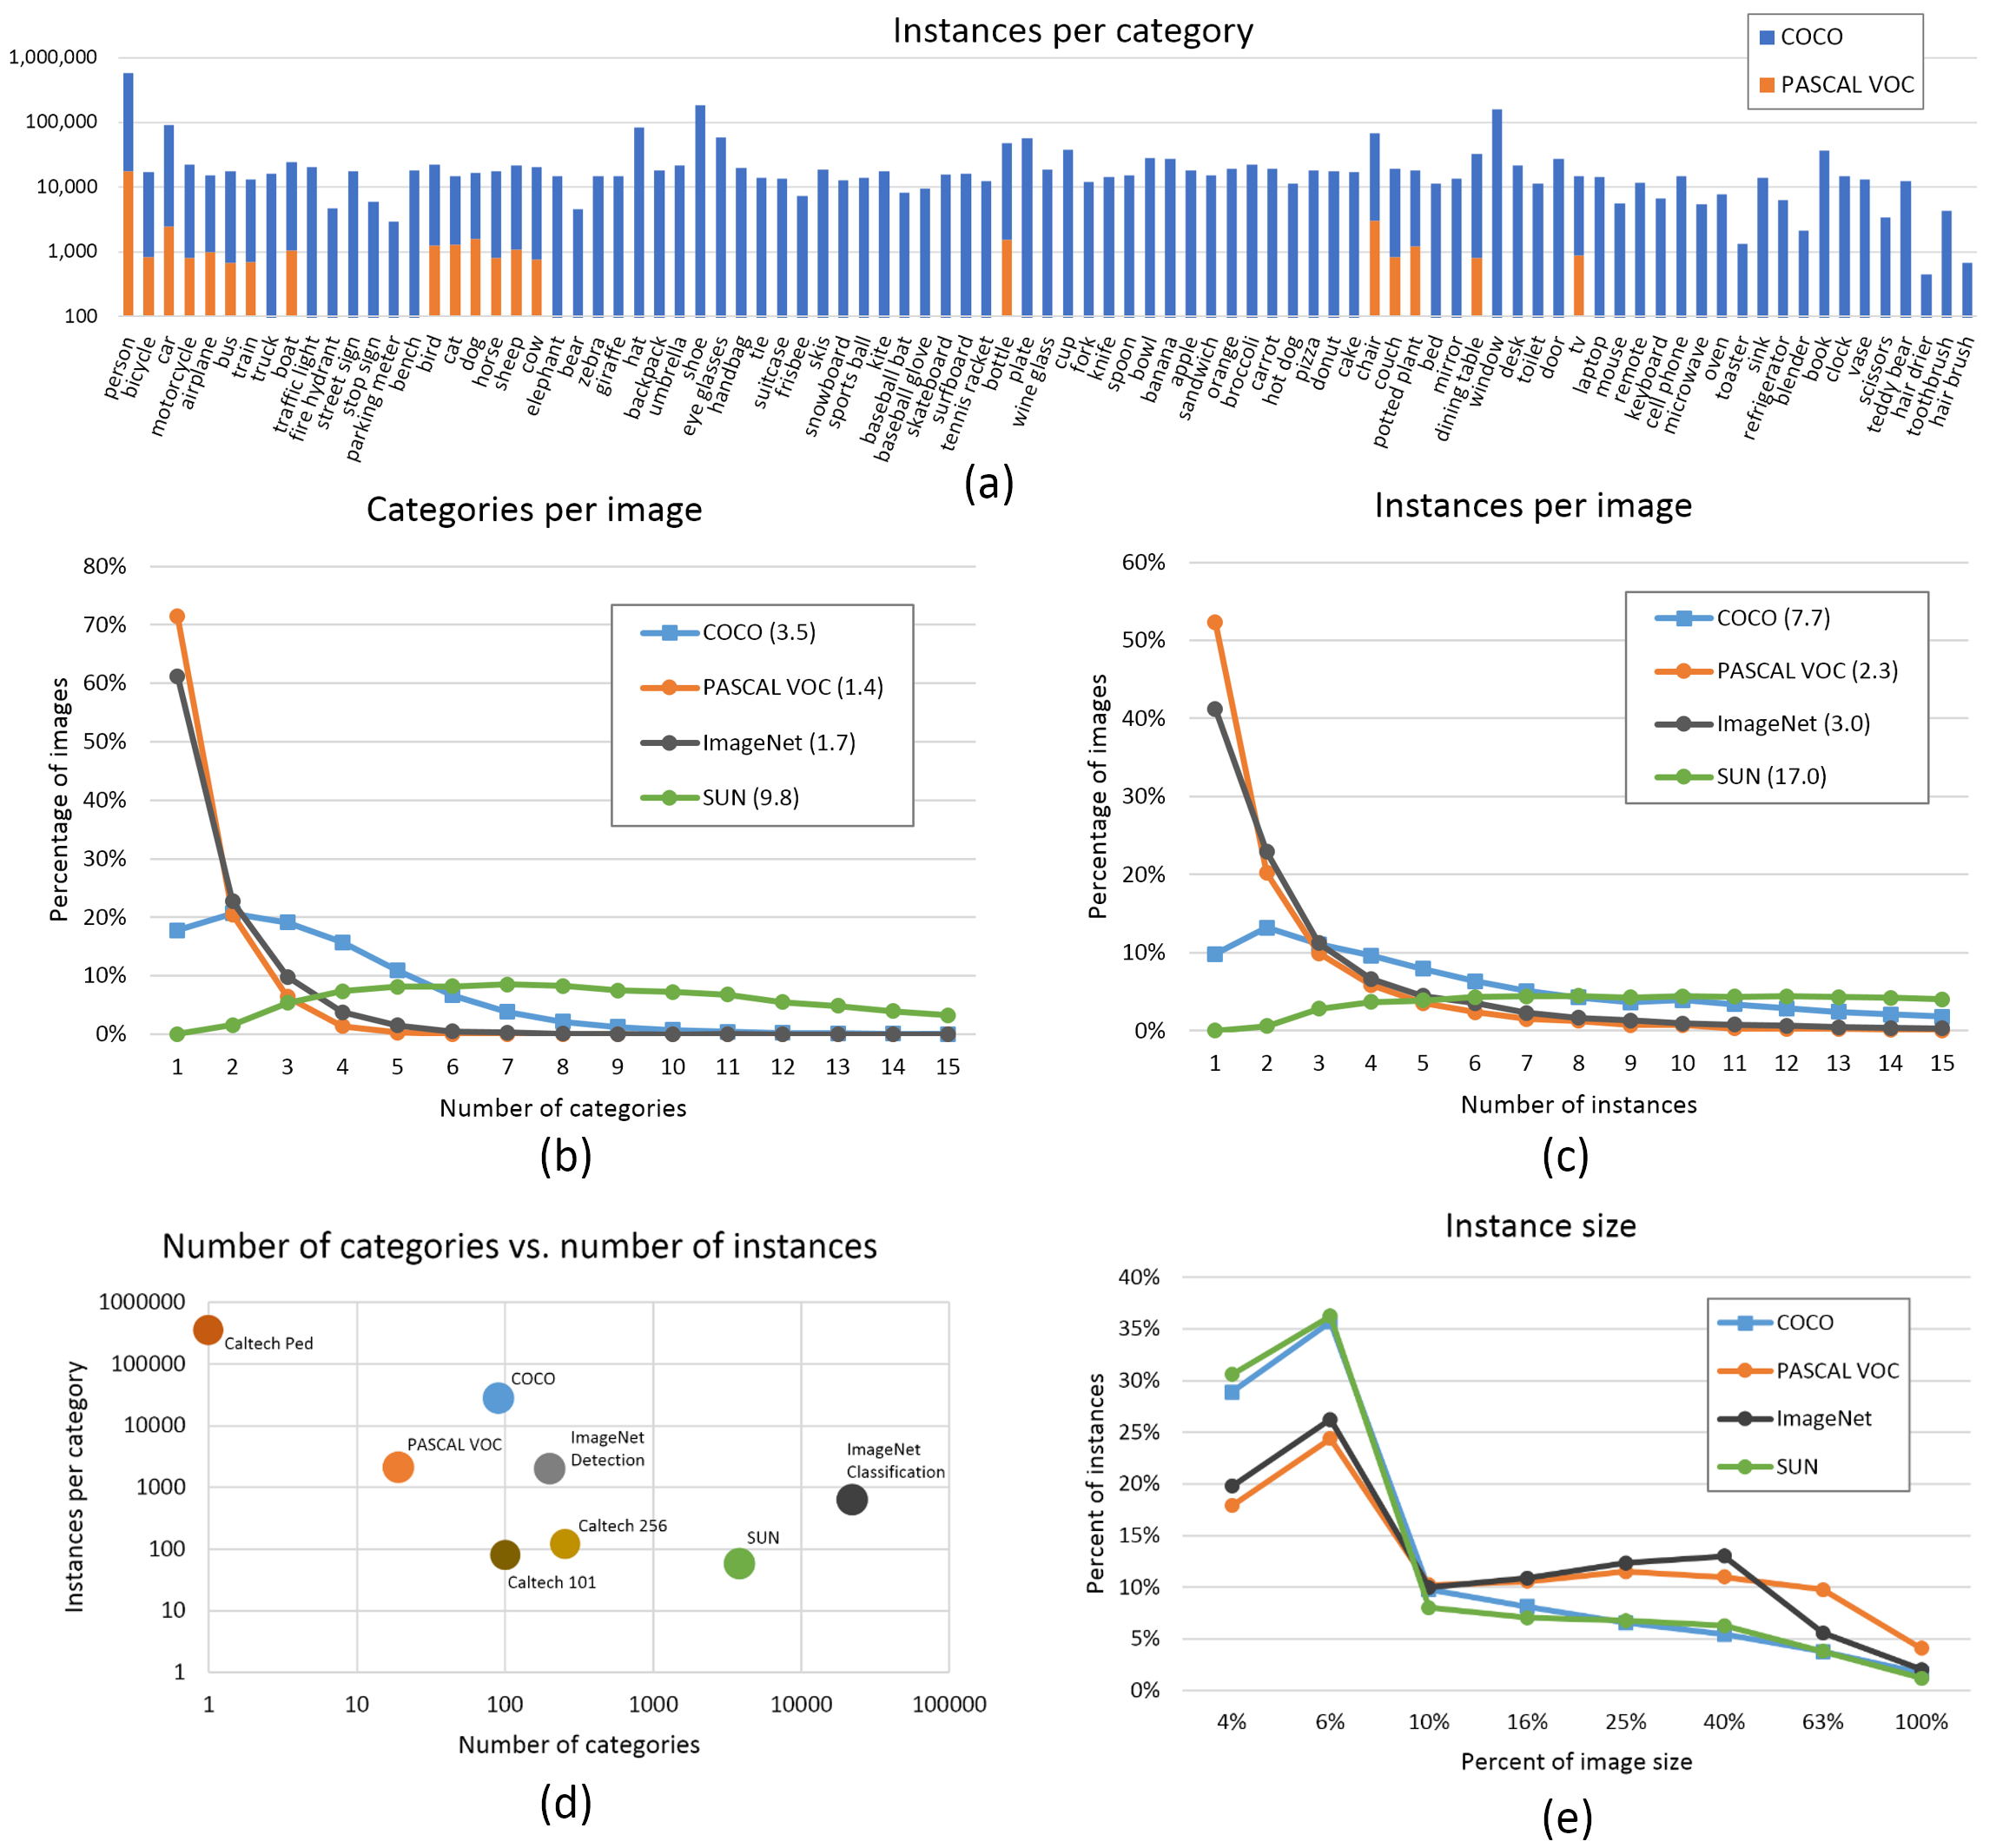
\includegraphics[width=\textwidth]{images/dataanalysis.png}
    \caption{Statistiche riassuntive di \ac{MSCOCO} \cite{lin2014microsoft}}
    \label{fig:dataanalysis_coco}
\end{figure}
\paragraph{Open Images} 
\ac{OID} \cite{krasin2017openimages}, nella versione 5, è un dataset composto da $9.2$ milioni di immagini. Ai giorni d'oggi rappresenta una delle sfide più interessanti insieme a \ac{ILSVRC} e \ac{MSCOCO}. Come per gli altri dataset anche questo si adatta a più task poiché le annotazioni sono state effettuate a livello di singola immagine, di \textit{object detection}, segmentazione e interazioni tra oggetti. 
Analizzando l'aspetto riguardante la rilevazione di oggetti ha ancora più classi rispetto a \ac{ILSVRC} in quanto per la si arriva a $600$ differenti label su $1.9$ milioni di immagini con \ac{BB} realizzate per la maggiorparte da annotatori professionali interni a Google. In aggiunta i contesti e le ambientazioni in cui sono s   tate catturate le immagini sono molto variegati.
\paragraph{EuroCity}  EuroCity è un dataset proposto da Braun \textit{et al. } nel 2019 \cite{braun2018eurocity}. Le immagini sono state acquisite da un veicolo in movimento in $31$ diverse città europee appartenentei $12$ differenti stati.
La risoluzione è di $1920 \times 1024$ con un framerate di $20$ immagini al secondo. Una particolarità delle immagini acquisite da queste telecamere è lo spazio colore che arriva a $16$ bit. Quest'alta gamma dinamica si traduce in una più alta qualità dei fotogrammi in condizioni di luce non ottimale, come può essere un controsole o una notturna. 
Per ogni città in media sono state catturate $1.7$ ore di video e le immagini sono state campionate ogni $4$ secondi ($80$ frame). Questo porta ad avere una ripetizione minore di pedoni o oggetti uguali, soprattutto in condizioni trafficate.

\subsection{Metriche}
\section{Detector basati su metodi tradizionali}
\label{sec:traditional_method}
\paragraph{VJ}
\paragraph{HOG}
\paragraph{DPM}
\section{Detector basati su Deep learning}
\label{sec:deep_learning_obj}
\subsection{Estrattori di feature}
\label{sec:feature_extractor}
\subsection{One Stage Detector}
\label{subsec:one_stage_detector}
\paragraph{YOLO}
\paragraph{SSD}
\paragraph{DSSD}
\paragraph{M2DET}
\paragraph{RefineNet}
\subsection{Two Stage Detector}
\label{subsec:two_stage_detector}
\paragraph{RCNN}
\paragraph{SPNNET}
\paragraph{FASTRCNN}
\paragraph{FASTERRCNN}
\paragraph{FPN}
\paragraph{MASKRCNN}
\section{RetinaNet}
\subsection{Focal Loss}